\chapter{Opis projektnog zadatka}
		
Cilj ovog projekta je razviti programsku podršku za stvaranje web aplikacije Dog Friendly koja će korisniku pomoći pronaći lokacije koje su prikladne i dostojne čovjekovog najboljeg prijatelja. Ova aplikacija  će vlasnicima i ljubiteljima pasa omogućiti pregled prikladnih i neprikladnih lokacija na interaktivnoj karti i time olakšati  druženje, igru i odmor.
Aplikacija  pruža i dodatak novih lokacija na interaktivnu kartu te za svaku novu lokaciju potrebno je dodatni nekoliko ključnih informacija poput imena lokacije, rating i kategorija( parkić, plaža, dućan, kafić, restoran, veterinarska
ambulanta, frizerski salon, itd.). Ako pritisnemo na indikator lokacije prikazat će nam se opis lokacije i kontakt. 
Korisnike ove aplikacije dijelimo na tri vrste:
\begin{packed_item}
	
	\item  neregistrirani korisnici
	\item  registrirani korisnici
	\item  vlasnici obrta
\end{packed_item}
\underbar{\textit{Neregistriranim korisnicima}} pružene su osnovne funkcionalnosti aplikacije(pregled interaktivne karte). 
\newline \underbar{\textit{Registrirani korisnici}} su korisnici koji su prošli kroz proces registracije koji se sastoji od 2 koraka. U prvom koraku korisnik ispunjava formu s:
\begin{packed_item}
	
	\item  korisničkim imenom
	\item   e-mail adresom
	\item  lozinkom
\end{packed_item}
%slika RegisterPage
\begin{figure}[H]
	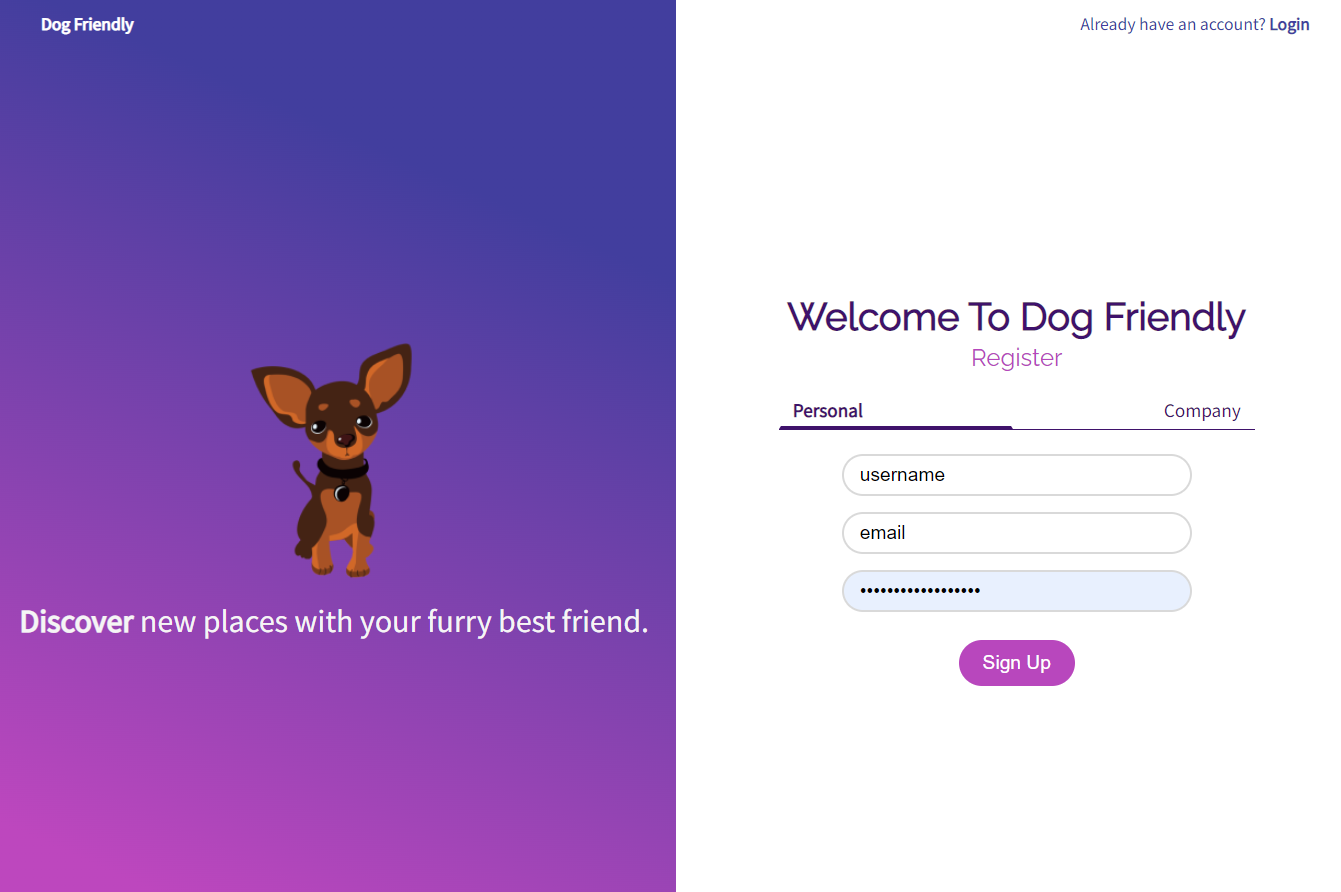
\includegraphics[scale=0.4]{slike/RegisterPage.png} 
	\centering
	\caption{Stranica za registraciju}
	\label{fig:promjene}
\end{figure}

Nakon ispunjavanja korisnik na svoju e-mail adresu prima obavijest o registraciji i traži ga se da potvrdi svoju registraciju. Nakon potvrde proces registracije je završen. Ako korisnik zaboravi svoju lozinku ili je dobio ideju za bolje korisničko ime pruža mu se promjena oba korisnička podatka. Registriranim korisnicima pružene su sve funkcionalnosti aplikacije koje imaju i neregistrirani korisnici uz priliku dodavanja novih lokacija na kartu. Osim toga, za već postojeće lokacije korisnik može potvrditi ili negirati njenu oznaku. 
\newline  \underbar{\textit{Vlasnici obrta}} moraju unijeti kroz dodatnu formu dodatne podatke:
\begin{packed_item}
	
	\item  naziv
	\item  adresu
	\item  OIB obrta
	\item  kontakt broj
	\item  kratki opis
	\item  kartični podatci
\end{packed_item} Financiranje aplikacije je zamišljeno putem reklama koje će vlasnici obrta moći izdati za određenu novčanu naknadu. Potvrdu o svakoj uplati korisnik će dobiti na svoju e-mail adresu.
\newline  Najpopularnije postojeće rješenje je BringFido u obliku web aplikacije i mobilne aplikacije dostupne u AppStoreu i na Google Playu. Na početnoj stranici odmah su ponuđene kategorije i tražilica koja nas dalje upućuje na poželjne informacije.
%slika homeFido
\begin{figure}[H]
	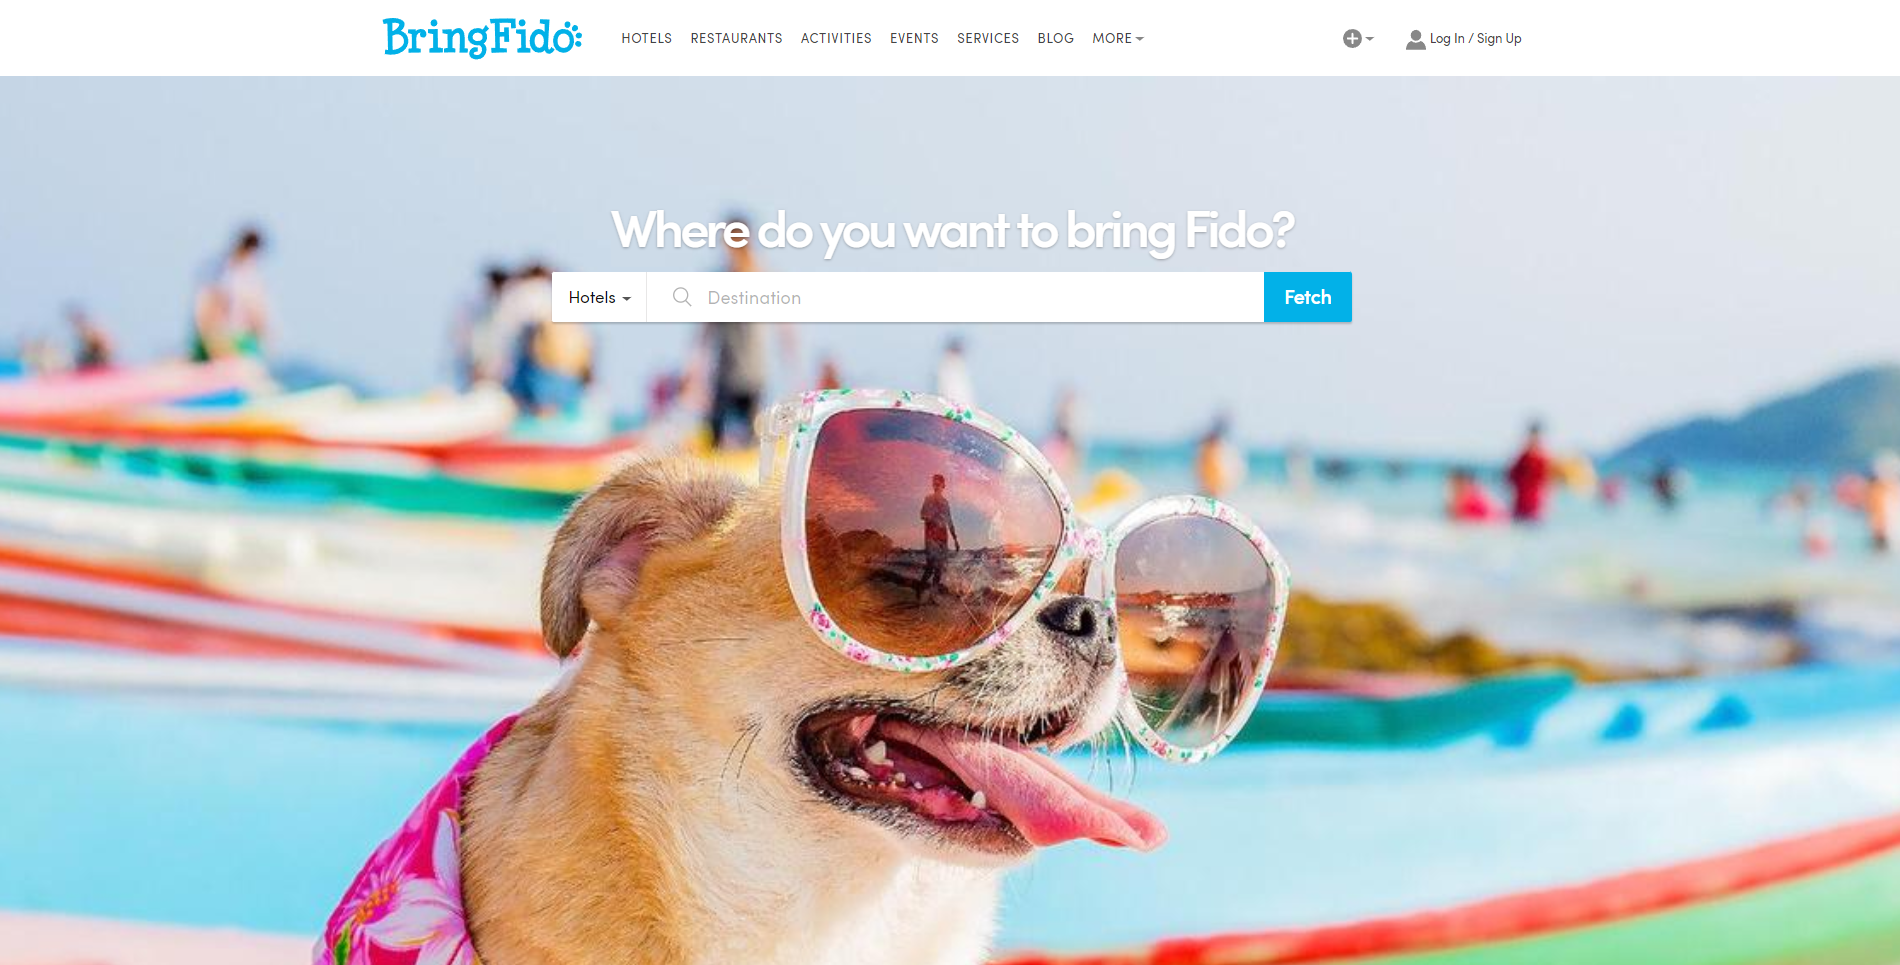
\includegraphics[scale=0.3]{slike/FidoHome.png} 
	\centering
	\caption{Početna stranica}
	\label{fig:promjene}
\end{figure}
Nove lokacije mogu dodati samo registrirani korisnici. Za lokaciju se prvo odabire kategorija kojoj pripada a zatim se ispunjavaju osnovne informacije o lokaciji. Za razliku od Dog Friendly na kraju se forma preda na pregled radnicima BringFidoa te ako se odobri bit će objavljena na njihovoj aplikaciji što znatno komplicira i usporava proces dodavanja lokacija no povećava kvalitetu sadržaja karte.
%bringFidobusiness
\begin{figure}[H]
	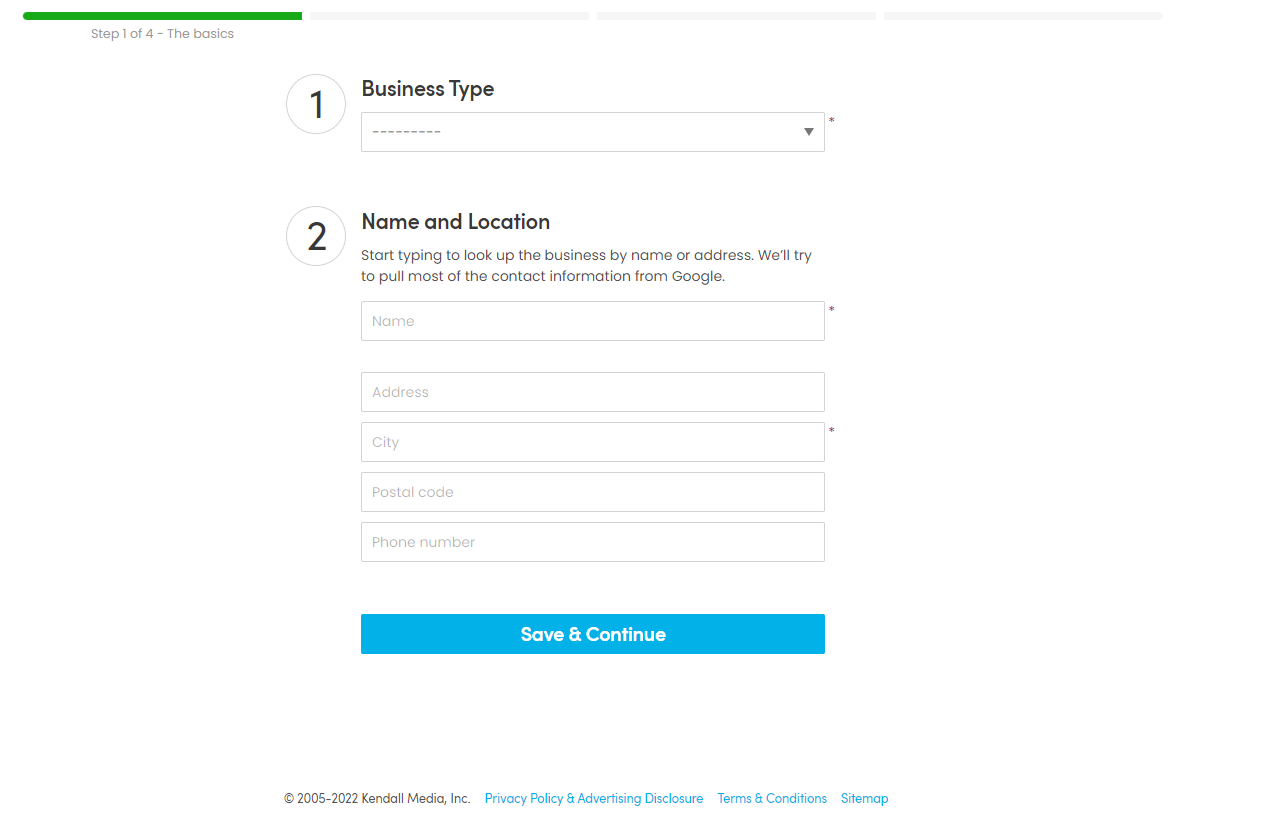
\includegraphics[scale=0.4]{slike/BringFidoBusiness.png} 
	\centering
	\caption{Primjer unosa novog obrta}
	\label{fig:promjene}
\end{figure}
Korisnici mogu ostaviti svoje komentare i iskustva o svakoj lokaciji, ali naravno i ocijeniti lokaciju. 
%fidoAddReview
\begin{figure}[H]
	
\includegraphics[scale=0.4]{slike/BringFidoAddReview.png}
	\centering
	\caption{Dodavanje osvrta}
	\label{fig:promjene}
\end{figure}
Još jedna značajna razlika je u sadržaju i jednostavnosti. BringFido sadrži previše nepotrebnih sadržaja koji nisu potrebni korisniku prilikom pretrage lokacija poput blogova vezanih uz kućne ljubimce.
%fidonNepotrebno
\begin{figure}[H]
	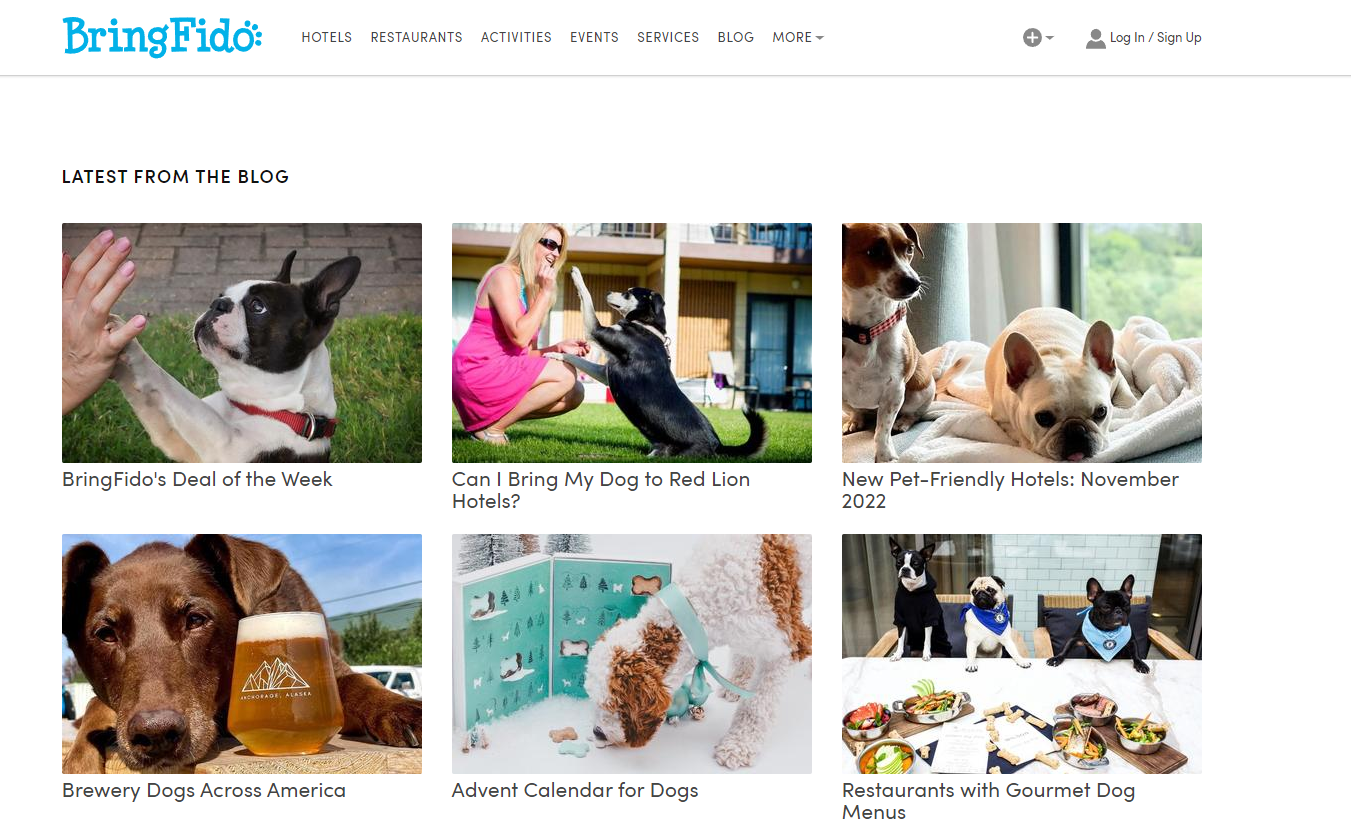
\includegraphics[scale=0.4]{slike/Nepotrebno.png}
	\centering
	\caption{Prikaz nepotrebnih sadržaja}
	\label{fig:promjene}
\end{figure}

\eject
		
	